\documentclass{article}
\usepackage{listings}
\usepackage{amsmath}
\usepackage{graphicx}
\usepackage{float}
\usepackage{subcaption}
\usepackage[linewidth=1pt]{mdframed}
\usepackage[colorlinks]{hyperref}

\usepackage{algorithm}
\usepackage{algpseudocode}

\usepackage{verbatim}

\hypersetup{citecolor=DeepPink4}
\hypersetup{linkcolor=DarkRed}
\hypersetup{urlcolor=Blue}

\usepackage{cleveref}

\setlength{\parindent}{1em}
\setlength{\parskip}{1em}
\renewcommand{\baselinestretch}{1.0}

\begin{document}

\begin{titlepage}
	\centering
	{\scshape\LARGE Progress Report\par}
	\vspace{1cm}
	{\scshape\Large Admissions data\par}
	\vspace{1.5cm}
	{\Large\itshape Javier Arechalde\par}
	\vfill
	{\large \today\par}
\end{titlepage}

\section{2000-2015 Data}

\subsection*{Original data}
 
In this section, we will analyze the different features available in the original dataset, and we will see which ones of them we can use or can't use, also which ones of them will be irrelevant to our classification task, even though we can use them.

\subsubsection*{Admit\_Term [2009, 2010,\dots, 2015] (categorical) CAN'T BE USED}

Year on which the student was admitted.

\subsubsection*{Admitted\_Semester [fall] (categorical) NOT RELEVANT}

The semester the student was admitted, we only have students that came in Fall so we won't be using this variable for our classification task.

\subsubsection*{ID [0,1, \dots] (categorical) NOT RELEVANT}

The student ID number. This variable is not relevant for our classification task.

\subsubsection*{Gender [male or female] (categorical)}

The student Gender.

\subsubsection*{Schoolname [New Bedford High School, \dots] (categorical)}

The student high school's name.

\subsubsection*{Schoolcity [New Bedford, Fall River, \dots] (categorical)}

The student high school's city.

\subsubsection*{Schoolcounty [Bristol, Berkshire, \dots] (categorical)}

The student's high school's county.

\subsubsection*{Schoolstate [MA,RI,NH, \dots] (categorical)}

The student's high school's state.

\subsubsection*{hsgpa [0-4] (numerical)}

The student's high school's GPA.

\subsubsection*{SATMA [200-800] (numerical)}

The student's math SAT score.

\subsubsection*{SATVB [200-800] (numerical)}

The student's verbal SAT score.

\subsubsection*{ACAD\_GROUP\_A [CAS,CNOW, \dots] (categorical)}

The college or program the student was admitted through.

\subsubsection*{Admitted\_major [ACT-BS, ACT-CP, \dots] (categorical)}

The major the student was admitted in.

\subsubsection*{ACAD\_GROUP\_C [CAS,CCB, \dots] (categorical)}

Current college or program the student is in.

\subsubsection*{Current\_Major [CIS-BS,BIO-BS] (categorical)}

The current major the student was studying.

\subsubsection*{ACAD\_GROUP\_D [CAS,CCB, \dots] (categorical) CAN'T BE USED}

The college the student graduated in. We can't use it as it would reveal if the student completed the program or not.

\subsubsection*{Degree\_Major [ACT-BS, ACT-CP, \dots] (categorical) CAN'T BE USED}

The major the student graduated with. We can't use it as it would reveal if the student completed the program or not.

\subsubsection*{Completion\_Term [2009,\dots,2015] (categorical) CAN'T BE USED}

The year the student completed his or her major. We can't use it as it would reveal if the student completed the program or not.

\subsubsection*{Completed\_Semester [Fall,\dots,Winter] (Categorical) CAN'T BE USED}

The semester the student completed the major. We can't use it as it would reveal if the student completed the program or not.

\subsubsection*{Completion [0 or 1] (categorical) PREDICTING VARIABLE}

This variable tells us if the student completed the program or not.


\subsection*{Dealing with missing data}

Some of the columns had missing values, so we decided to fill the missing values in these rows with the average value of each one of this features. So for the following features, what we did is to select the column containing this feature, then get rid of the missing values in this column and calculate the mean of the remaining values. Afterwards, we replaced those missing values with the mean that calculated that way.

\begin{itemize}
 \item High school GPA
 \item SATMA
 \item SATVB
\end{itemize}

Another columns, like \textit{Current\_Major} had a lot of missing values too, so we supposed that if there was a missing value in that column, the student didn't change his or her major.

\subsection*{Derived features}

We added some more features to our dataset, to try to enrich it and make it more meaningful. Here are the different features that we added to our dataset.

\subsubsection*{Distance}

We used a library for $R$ called \textit{gmapsdistance} that uses Google Maps to calculate the distance s and the time distance between two cities. We calculated the distance in miles, and in minutes driving from Umass Dartmouth to that student's high school city.

\subsubsection*{Total SAT}

We calculated the total SAT for each student by simply adding the verbal SAT and math SAT.

$$TotalSAT = SATMA+SATVB$$

\subsubsection*{Honors Student}

We created a column that tells us if the student graduated with honors in his or her High School or not, by simply checking if this student's high school GPA was equal or greater than $4$.

\subsubsection*{Above GPA or SAT}

Then we created another two features to see if the student was a student is an above average student or not, depending on the GPA and total SAT.

\subsubsection*{Location}

In this column, we stored some information related to the student location. We separated the students in this different classes.

\begin{itemize}
 \item Student is from MA and Bristol county
 \item Student is from MA but not from Bristol
 \item Student is from some of the states adjacent to MA
 \item Student is from another state that is not MA or adjacent to MA
 \item Student is from outside the US
\end{itemize}

\subsubsection*{Changed Major}

We added a column that indicated if the student changed his or her major or not, we could do this by comparing the admitted major column, with the currrent major column. If the value in current major was different from the one in admitted major, we considered that the student changed his major, otherwise he or she did not.

\subsubsection*{Income}

We wanted to try to include some finantial information in the dataset, so we used another dataset that we found in the Federal Government website, that includes the average household income for different counties. So for each of the students, we matched the student's high school county to the county in this dataset, and added the corresponding average household income for that county into our dataset.

\subsubsection*{Direct Admission}

In this column, we determine if the student was directly admitted into school, or if the student came into school through a PCE or College Now or a pathway program.

\subsubsection*{Performance Groups}

We also separated the students into different performance groups: high, average, and low. Depending on how is their SATMA, SATVB or GPA compared to different students in his or her same high school, county or region.

\subsection*{Normalization}

In order to help our machine learning algorithm with the classification task, we normalized all the numerical features, so all this features will be in a range from 0 to 1. We used this formula to change the range, the maximum and minimum values are the maximum and minimum values of that feature in the dataset:

$$newvalue = \frac{oldvalue-min}{max-min}$$

\section*{Fall 2011 Retention Cohort Data}

The second dataset that was provided, was a superset of the first dataset, it included the same variables as the first one, but also a lot of new variables that could be useful for our classification task, like the age of the student, the number of courses the student took when he registered in fall, the student zipcode, etc.

It also included data from every year, like the postal zip the second year the student was in the school, which could tell us if the student changed his residency or not, we could also see the number of courses the student was taking every single semester, etc. since the student came to school, until the student graduated (or not). The main issue here is that whenever we want to predict if a student is going to graduate at UMassD or not, we won't have any on this information available, we can only use the variables from when the student first came to school. The only scenario in which we could use those variables is if we wanted to do some exploratory analysis to try to find out when the student left the school, and see if there is any pattern before this happened.

Another issue that we faced with this dataset, is that we only have around 500 rows, so when running a classification task, like AdaBoost, the results are not consistent, due to the reduced number of items in the training and test set.

\section*{Models}

For the classification task, we tried different machine learning algorithms in $R$ to see which one of them could give us the best results.

\subsection*{Decision Trees}

Decision trees was the first model we tried, and as it is the simplest one here it was also the one with the lowest performance, so we though that it wasn't worth the effort to continue trying to push the limits of this model, as it didn't seem we were going to get a good performance by tuning it.
                     
\subsection*{Random forest}

Then we tried \textit{Random Forest}, which is a derived model from Decision Trees, that uses a combination of them to get better results. We tuned the model to find the number of trees that gave us the best performance, by analyzin the \textit{Out Of Bag} error \textit{OOB}. We saw that the OOB error wasn't decreasing after $300$ trees, so we decided to set the number of trees for Random Forest to this number. This method gave us fairly good results, but another model (AdaBoost) gave us better results, so we decided to leave this model aside for the moment, but it'll be probably be worth revisiting to see how good it can perform, if we push its limits.

The main issue with this model, is that can't handle features that contain $NA$ values, nor handle features that have more than $53$ categories, so we can't use for example the school name or the school city as a feature for the prediction, as there are more than $53$ different school names and school cities in our dataset.

\subsection*{SVM}

We also tried Support Vector Machine to see how well it performed. At first we used linear kernel, but the model could only classify the test sample as a '0' class. By using a \textit{Gaussian} kernel, we were able to have a good performance, the main problem with this model was that it is not able to handle missing data, so we can't classify the samples that have any missing value in the features that we chose for our model, so we decided not to go with this model.

\subsection*{Adaboost}

Adaboost was the model that was giving us the best results from the beginning, as it is a machine learning algorithm suitable for binary classification tasks that uses a combination of weak classifiers. As we just want to classify the students in two groups, the ones that are graduating, and the ones that are not, we decided to go with it. 

We first got rid of the students that came in a year later from 2011 from the dataset, because those students may be still studying in the school, and therefore haven't graduated yet so we can't use that data. 

We then partitioned the dataset into training and test set (70\%, 30\%) and we trained our model using all the features that we could use from the dataset with the features we added, using the train set, and a 100 iterations. In this case, we can get a performance of around 75\%. The problem with this is that we can get this really good performance because when training the model, we use data from all the different Admit\_Term in the dataset (the year the student came into school), so when we try to classify a new student we already have data from that year, but in a real life situation we won't have data for the year the student came in, so we have to try a different test.

Here is the confusion matrix for this 

\begin{figure}[H]
\begin{center}
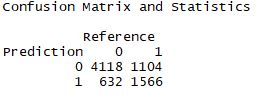
\includegraphics[scale=1]{Conf1}
\end{center}
\caption{Confusion Matrix 1}
\end{figure}

Instead, we will create a train partition using data from 4 consecutive years in the school, and for the test set, we can use the next two years after those 4 consecutive years, that will be the closer we can get to a real life situation, when trying to predict if a new student will graduate or not. In this case, we get an accuracy around 60\% training the Adaboost model with 100 iterations.

\begin{figure}[H]
\begin{center}
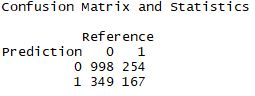
\includegraphics[scale=1]{Conf2}
\end{center}
\caption{Confusion Matrix 2}
\end{figure}

\subsection*{Conclusions}

We tried different machine learning algorithms for this classification task. We found out that two of them were clearly outperforming the rest, that is \textit{RandomForest}, and \textit{AdaBoost}. We tuned this models to try to obtain the best performance possible, and we found out that, with the data we have avaliable right now, \textit{Adaboost} is the best possible model, as it can handle missing values, and it can also handle features that contain more than $53$ different categories.  

We also tried adding some features that we derived form the ones that already were in the dataset, to see if we can improve the model's performance, but unfortunately, we still couldn't add a feature that really helped our classification task. There are still some features derived from the location of the student that could be added to our dataset, like if there are school in the student's area that could be the student's first choice instead of UmassD.

We also tried to add data from other datasets, like the one from the \textit{United States Census Bureau}, that contains the average household income per county. These datasets can be found \href{https://www.census.gov/support/USACdataDownloads.html}{here}. Unfortunately this data didn't help our model to better classify the students, probably because most of the students are from MA, so we have few different counties. If we had more data from the second dataset, which includes the zipcode too, we could use it to get the average household income per zipcode instead of the county, which will probably be more accurate.

The features that helped the most our classification task were the \textit{Admit\_Term}, or the year the student came to school, the location related features, and the major or college inside the school the student was enrolled in. 

To summarize this last section, in my opinion, the direction that we should take from here is to use \textit{Adaboost} as our machine learning algorithm, with a dataset like the second one that was provided (The Fall 2011 Retention Cohort Data), but with more rows. This second dataset has all the features in the first dataset, and also some extra features that could be really useful.

\end{document}
